% Tipo di documento.
\documentclass[a4paper ,openright]{report}
% Dimensione dei margini
\usepackage[a4paper,top=3cm,bottom=3cm,left=3cm,right=3cm]{geometry} 
% Dimensione del font
\usepackage[fontsize=13pt]{scrextend}
% Lingua del testo
\usepackage[english,italian]{babel}
% Codifica del testo
\usepackage[utf8]{inputenc} 
% Encoding del testo
\usepackage[T1]{fontenc}
% Permette di generare testo fittizio. Mi è stato utile 
% per capire quale sarebbe stata l'impostazione del 
% testo nella pagina prima che scrivessi un determinato paragrafo
\usepackage{lipsum}
% Per ruotare le immagini
\usepackage{rotating}
% Per modificare l'header delle pagine 
\usepackage{fancyhdr}
% Librerie matematiche
\usepackage{amssymb}
\usepackage{amsmath}
\usepackage{amsthm}         

% Uso delle immagini
\usepackage{graphicx, wrapfig}
% Uso dei colori
\usepackage[dvipsnames]{xcolor}         
% Uso dei listing per il codice
\usepackage{listings}          
% Per codice VHDL
\usepackage{minted}
% Per inserire gli hyperlinks tra i vari elementi del testo 
\usepackage{hyperref}     
% Diversi tipi di sottolineature
\usepackage[normalem]{ulem}

% Chapter con barra verticale
\usepackage[T1]{fontenc}
\usepackage{titlesec, blindtext, color}
\definecolor{gray75}{gray}{0.75}
\newcommand{\hsp}{\hspace{20pt}}
\titleformat{\chapter}[hang]{\Huge\bfseries}{\thechapter\hsp\textcolor{gray75}{|}\hsp}{0pt}{\huge\bfseries}
% -----------------------------------------------------------------

% Modifica lo stile dell'header
\pagestyle{fancy}
\fancyhf{}
\lhead{Prova Finale Progetto di Reti Logiche}
\rhead{\textbf{\thepage}}
\fancyfoot{}
\setlength{\headheight}{12.5pt}

% Rimuove il numero di pagina all'inizio dei capitoli
\fancypagestyle{plain}{
  \fancyfoot{}
  \fancyhead{}
  \renewcommand{\headrulewidth}{0pt}
}

% Stile del codice
\lstdefinestyle{codeStyle}{
    % Colore dei commenti
    commentstyle=\color{teal},
    % Colore delle keyword
    keywordstyle=\color{Magenta},
    % Stile dei numeri di riga
    numberstyle=\tiny\color{gray},
    % Colore delle stringhe
    stringstyle=\color{violet},
    % Dimensione e stile del testo
    basicstyle=\ttfamily\footnotesize,
    % newline solo ai whitespaces
    breakatwhitespace=false,     
    % newline si/no
    breaklines=true,                 
    % Posizione della caption, top/bottom 
    captionpos=b,                    
    % Mantiene gli spazi nel codice, utile per l'indentazione
    keepspaces=true,                 
    % Dove visualizzare i numeri di linea
    numbers=left,                    
    % Distanza tra i numeri di linea
    numbersep=5pt,                  
    % Mostra gli spazi bianchi o meno
    showspaces=false,                
    % Mostra gli spazi bianchi nelle stringhe
    showstringspaces=false,
    % Mostra i tab
    showtabs=false,
    % Dimensione dei tab
    tabsize=2
} \lstset{style=codeStyle}

% Stile di codice per dimensioni maggiori, in cui ho avuto bisogno di un testo più piccolo (ad esempio se si vuole inserire del codice che ha linee molto lunghe). Per usare questo stile piuttosto che il precedente, usare 

% \lstset{style=longBlock}
%  % inserire il codice...
% \lstset{style=codeStyle}

% Il secondo comando consente di tornare allo stile precedente 
\lstdefinestyle{longBlock}{
    commentstyle=\color{teal},
    keywordstyle=\color{Magenta},
    numberstyle=\tiny\color{gray},
    stringstyle=\color{violet},
    basicstyle=\ttfamily\scriptsize,
    breakatwhitespace=false,         
    breaklines=true,                 
    captionpos=b,                    
    keepspaces=true,                 
    numbers=left,                    
    numbersep=5pt,                  
    showspaces=false,                
    showstringspaces=false,
    showtabs=false,                  
    tabsize=2
} \lstset{style=codeStyle}

% Margini prima e dopo blocchi di codice, per avere più distanza
\lstset{aboveskip=20pt,belowskip=20pt}

% Aggiunti definizioni, teoremi, linea e listing
\newtheorem{definition}{Definizione}[section]
\newtheorem{theorem}{Teorema}[section]
\providecommand*\definitionautorefname{Definizione}
\providecommand*\theoremautorefname{Teorema}
\providecommand*{\listingautorefname}{Listing}
\providecommand*\lstnumberautorefname{Linea}

\raggedbottom



% -----------------------------------------------------------------
\begin{document}

\begin{titlepage}
\begin{figure}[!htb]
    \centering
    
\includegraphics[keepaspectratio=true,scale=1.5]{images/Frontespizio/pol.eps}
\end{figure}

\begin{center}
    \huge{Politecnico di Milano}
    \vspace{10mm}
    \\ \Large{Laurea Triennale in Ingegneria Informatica}
\end{center}
\vspace{35mm}
\begin{center}
    {\LARGE{\bf Prova Finale Progetto di Reti Logiche }}
\end{center}
\vspace{70mm}

\begin{minipage}[t]{0.47\textwidth}
	{\large{Professore:}{\normalsize\vspace{3mm}
	\bf\\ \large{William Fornaciari}}}
\end{minipage}
\hfill
\begin{minipage}[t]{0.47\textwidth}\raggedleft
	{\large{Studente:}{\normalsize\vspace{3mm} \bf\\ \large{Paolo Cerutti}}}
\end{minipage}

\vspace{10mm}
\hrulefill
\\\centering{\large{ANNO ACCADEMICO 2021/2022}}

\end{titlepage}

\tableofcontents

\chapter{Introduzione}
La specifica della \textit{Prova Finale (Progetto di Reti Logiche)} 2021/2022 richiede di 
implementare un modulo Hardware descritto in VHDL che si interfacci con una
memoria con l'obiettivo di rappresentare un codificatore convoluzionale con tasso di trasmissione \( \frac{1}{2} \).
\section{Specifica del progetto}
Il modulo da implementare deve leggere la sequenza da codificare da una memoria, applicare la convoluzione parola per parola e 
successivamente salvare in memoria la sequenza codificata.
In particolare, dato un ordine, dovrà:
\begin{enumerate}
    \item Leggere la quantità di parole da codificare dalla memoria;
    \item Leggere la sequenza di parole da codificare una alla volta dalla memoria, ogni singola parola di memoria è un Byte;
    \item Trasformare la sequenza di Byte in un flusso di Bit (Serializzazione);
    \item Applicare al flusso di Bit il codice convoluzionale;
    \item Generare in uscita un flusso di Bit;
    \item Trasformare il flusso di Bit in Byte (Parallelizzazione);
    \item Salvare in memoria il risultato.
\end{enumerate}
Il tasso di trasmissione \( \frac{1}{2} \) indica che un Bit viene codificato con due Bit; infatti, il flusso 
in uscita è ottenuto come concatenamento alternato dei due Bit di uscita.

Il convolutore è una macchina sequenziale sincrona con un clock globale e un segnale di reset avente il diagramma 
degli stati come in \autoref{fig:Convolutore} e che ha nel suo 00 lo stato iniziale.
\begin{figure}
    \centering
    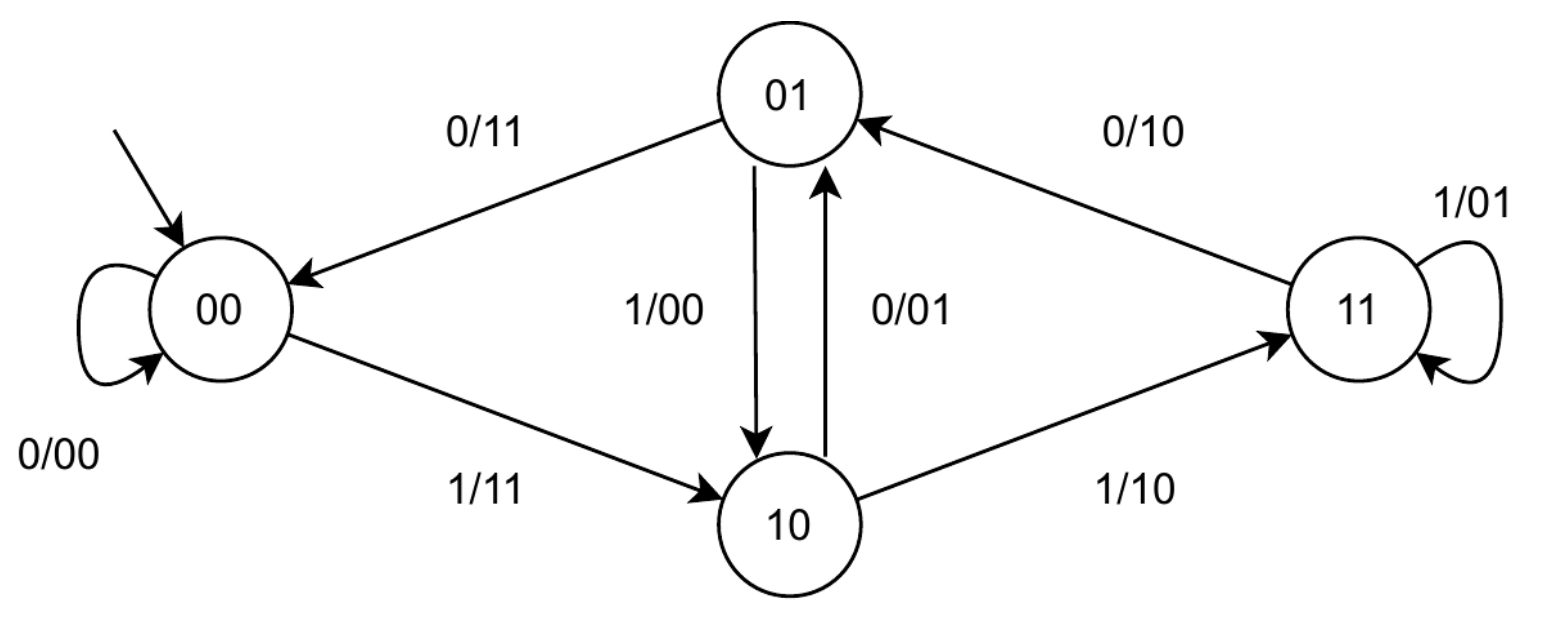
\includegraphics[width= 0.8\textwidth]{images/Capitolo1/conv.png} 
    \caption{Macchina a stati del codificatore convoluzionale} 
    \label{fig:Convolutore}
\end{figure}
\newpage
\section{Dati e dettagli}
\begin{itemize}
    \item Il modulo partirà nell'elaborazione quando un segnale \texttt{START} in ingresso verrà portato a 1.
    \item Il segnale di \texttt{START} rimarrà alto fino a che il segnale di \texttt{DONE} non verrà portato a 1.
    \item Al termine della computazione, il modulo da progettare deve portare a 1 il segnale \texttt{DONE} che notifica la fine dell’elaborazione e deve rimanere alto finché il segnale di \texttt{START} non è riportato a 0. 
    \item Un nuovo segnale \texttt{START} non può essere dato finché \texttt{DONE} non è stato riportato a 0. Se a questo punto viene rialzato il segnale di \texttt{START}, il modulo dovrà ripartire con la fase di codifica.
    \item Il modulo deve essere dunque progettato per poter codificare più flussi uno dopo l’altro. Ad ogni nuova elaborazione, il convolutore viene portato nel suo stato di iniziale 00.
    \item Il modulo deve essere progettato considerando che in una seconda elaborazione non dovrà attendere il \texttt{RESET} del modulo ma solo la terminazione dell'elaborazione.
\end{itemize}

\section{Struttura memoria}
La quantità di parole da codificare è memorizzata nell’indirizzo 0; il primo Byte (quindi la prima parola) della sequenza è memorizzato all’indirizzo 1. Le parole codificate in uscita devono essere memorizzate a partire dall’indirizzo 1000. La dimensione massima della sequenza di ingresso è 255 Byte.

\section{Interfaccia componente}
Il componente da descrivere ha un’interfaccia così definita:
\inputminted{vhdl}{listings/Capitolo1/componente.vhd}
In particolare:
\begin{itemize}
    \item \texttt{i\_clk} è il segnale di \texttt{CLOCK} in ingresso generato dal testbench;
    \item \texttt{i\_rst} è il segnale di \texttt{RESET} che inizializza la macchina pronta per ricevere il primo segnale di \texttt{START};
    \item \texttt{i\_start} è il segnale di \texttt{START} generato dal testbench;
    \item \texttt{i\_data} è il segnale che arriva dalla memoria in seguito ad una richiesta di lettura;
    \item \texttt{o\_address} è il segnale di uscita che manda l’indirizzo alla memoria;
    \item \texttt{o\_done} è il segnale di uscita che comunica la fine dell’elaborazione e il dato di uscita
    \item \texttt{o\_en} è il segnale di \texttt{ENABLE} da dover mandare alla memoria per poter comunicare
(sia in lettura che in scrittura);
    \item \texttt{o\_we} è il segnale di \texttt{WRITE ENABLE} da dover mandare alla memoria per poter scriverci. Per leggere da memoria esso deve essere 0;
    \item \texttt{o\_data} è il segnale di uscita dal componente verso la memoria.
scritto in memoria;
\end{itemize}
\chapter{Architettura}
\section{Approccio problema}
Si è deciso di approcciare il problema con una macchina a stati finiti. Trattandosi di un problema di complessità ridotta si è optato per una soluzione mono modulare con un singolo process che elabora i vari stati.

\section{Macchina a stati}
Di seguito una breve spiegazione degli stati della macchina e i segnali di controllo:
\begin{wrapfigure}{r}{0.50\textwidth}
    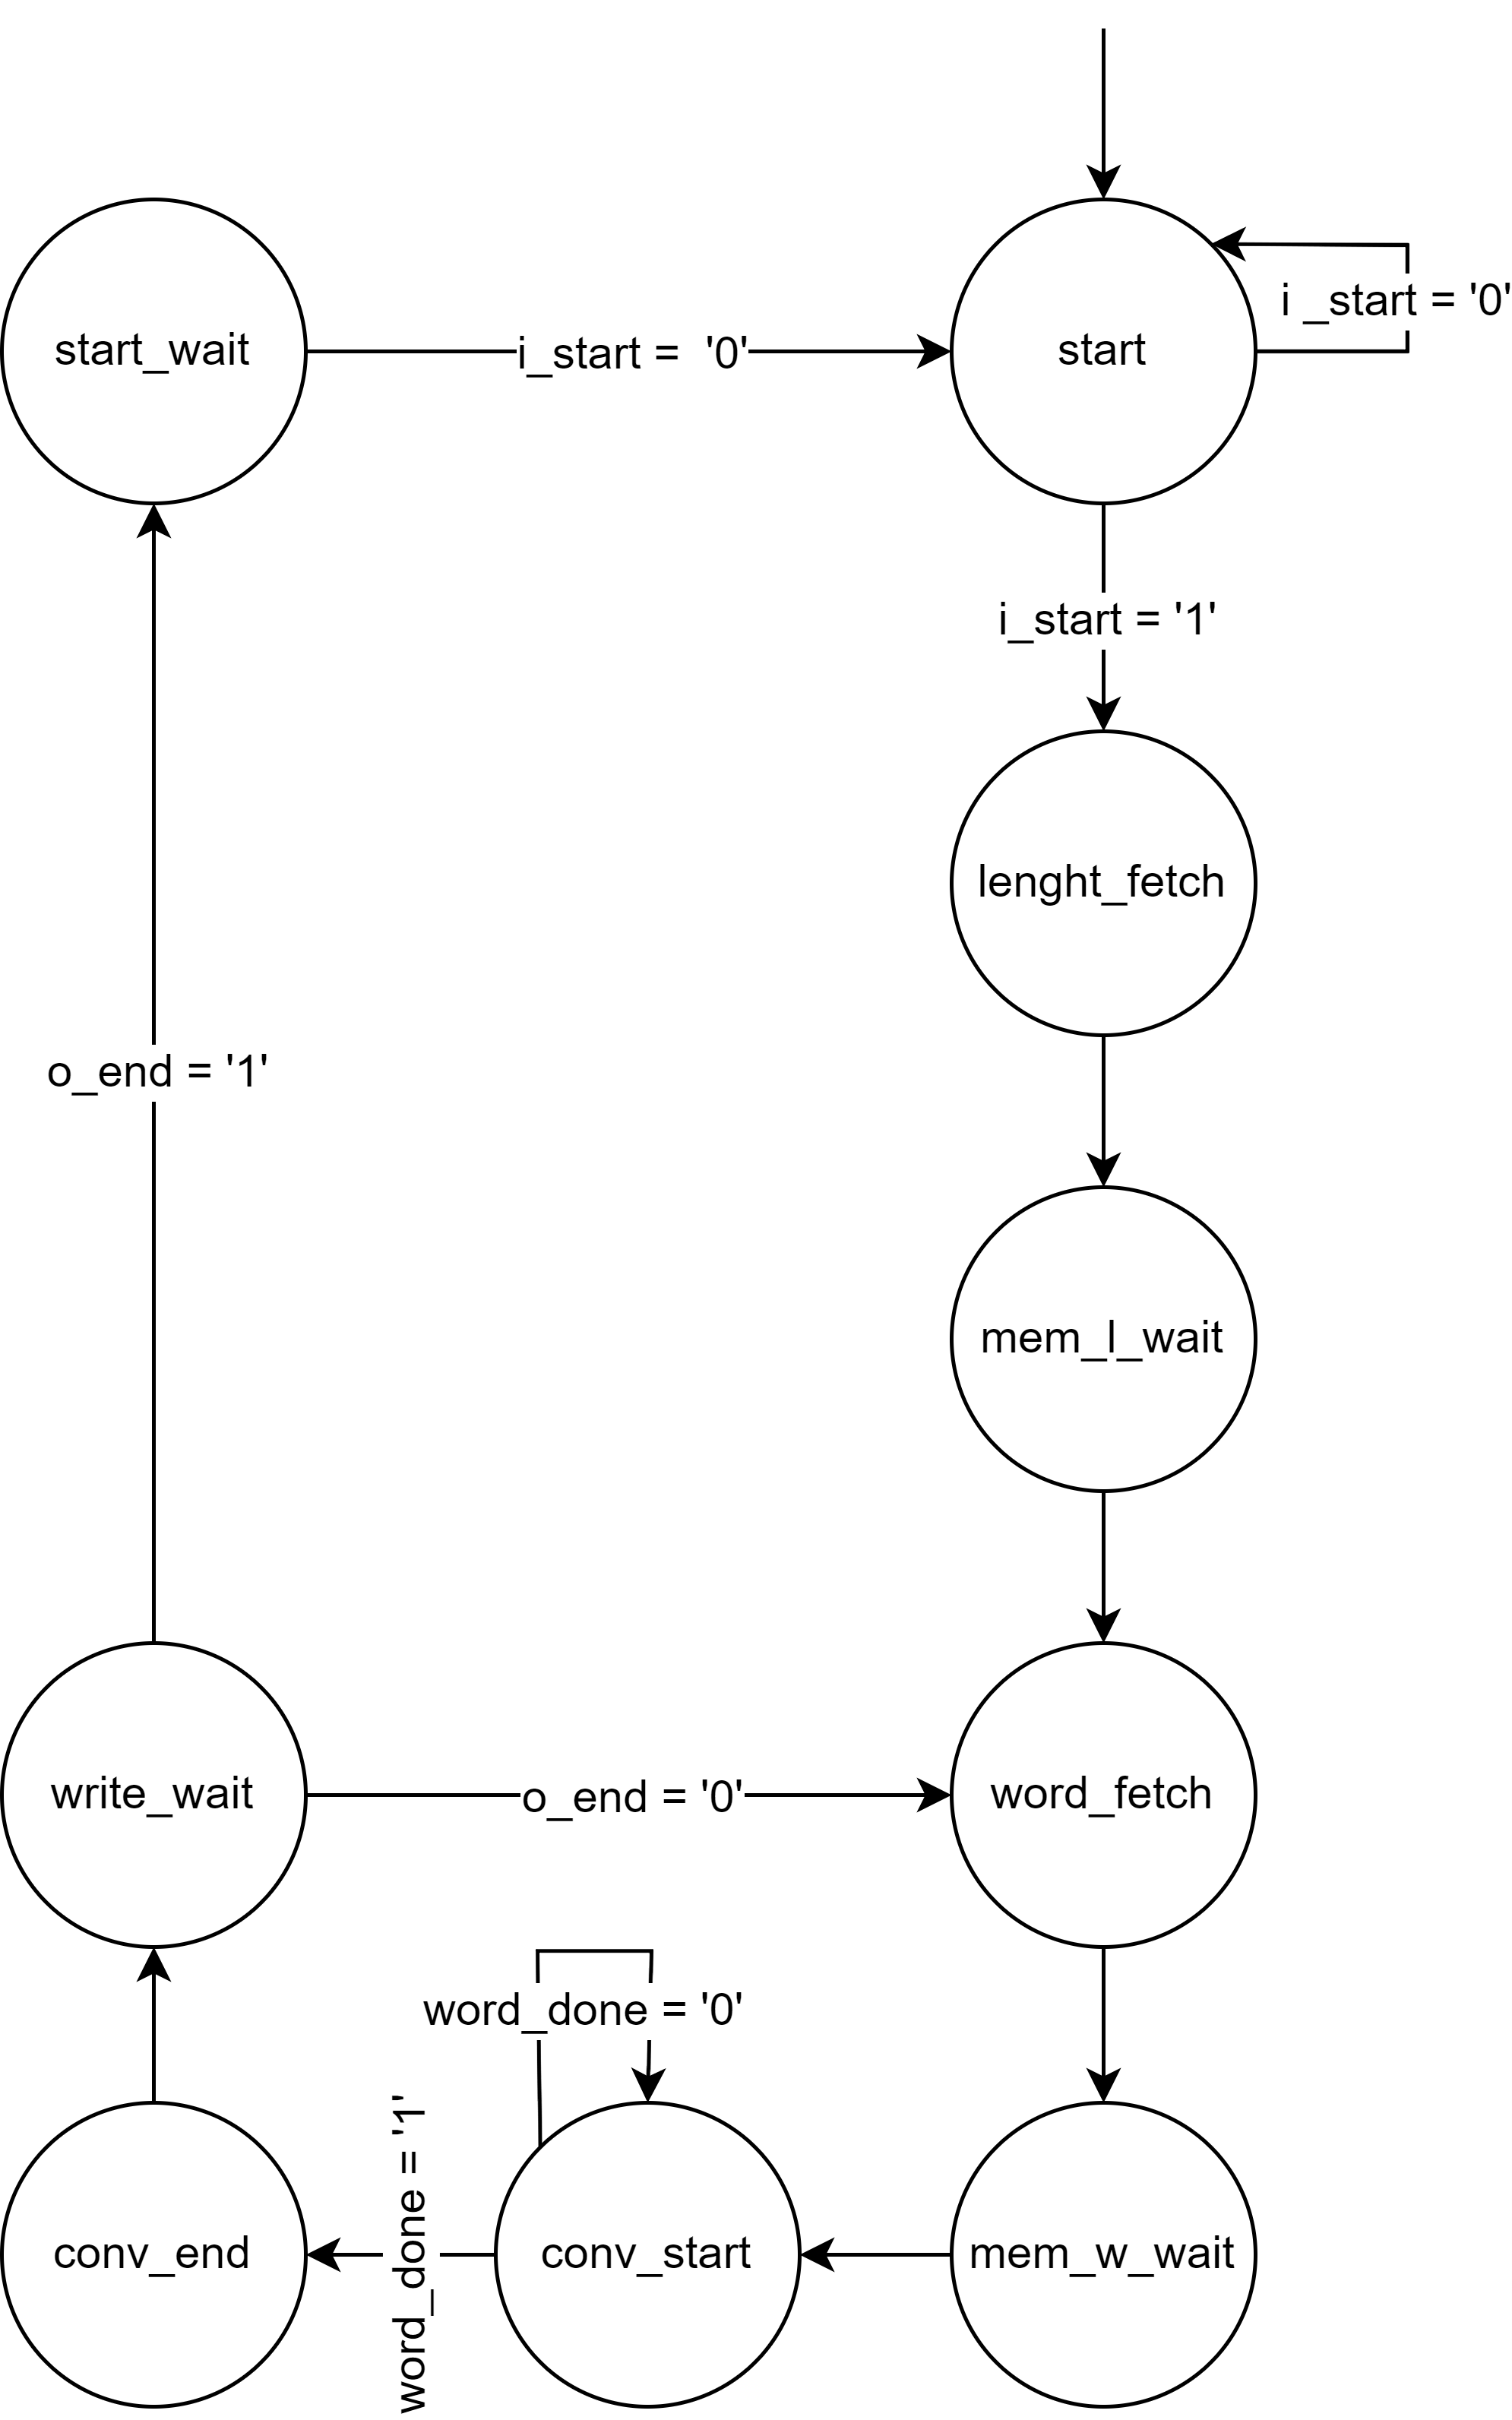
\includegraphics[trim=0cm 40cm 0cm 6.7cm, width=0.50\textwidth]{images/Capitolo2/vertical_fsm.png}
\end{wrapfigure}
\begin{itemize}
    \item \texttt{start}: Lo stato di inizio, è anche lo stato di reset. In questo stato si aspetta che il segnale \texttt{i\_start} venga alzato a 1.
    \item \texttt{length\_fetch}: Lo stato in cui vengono alzati i segnali per poter leggere dalla memoria, in particolare la lunghezza della parola.
    \item \texttt{mem\_l\_wait}: Lo stato di attesa per permettere alla memoria di caricare il dato.
    \item \texttt{word\_fetch}: Lo stato in cui vengono alzati i segnali per poter leggere dalla memoria, in particolare la parola.
    \item \texttt{mem\_w\_wait}: Lo stato di attesa per permettere alla memoria di caricare il dato.
\end{itemize}

\begin{itemize}
    \item \texttt{conv\_start}: Lo stato in cui viene eseguita la serializzazione e la codifica della parola. La macchina rimane in questo stato fino a quando \texttt{word\_done} viene posto a 1.
    \item \texttt{conv\_end}: Lo stato in cui la codifica è conclusa e inizia il processo di scrittura in memoria. (Primi Byte)
    \item \texttt{write\_wait}: Lo stato in cui termina il processo di scrittura in memoria (Secondo Byte).
    \item \texttt{start\_wait}: Lo stato di arrivo se la macchina ha codificato tutte le parole.
\end{itemize}

\section{Algoritmi implementati}
Di seguito una breve spiegazione della logica implementata per poter affrontare i problemi di serializzazione e parallelizzazione e di codifica delle parole.
\subsubsection{Serializzazione}
La serializzazione della parola si basa sull'utilizzo di shift. Infatti, quando necessario, viene salvato in un \texttt{std\_logic} il bit nella posizione più significativa della parola da codificare (che è salvata in un \texttt{std\_logic\_vector}); dopodiché al vettore viene effettuato uno shift una posizione verso sinistra, così che sia pronto per il prossimo ciclo.

\subsubsection{Codifica della parola} \label{codifica}
Supponendo che il bit da codificare sia chiamato \( msg \), i bit in output siano chiamati rispettivamente \( x_1 \) e \( x_0 \)\footnote{ \( x_1 \) è il bit più significativo rispetto a \( x_0 \)} e la bitmask dello stato corrente della macchina del convolutore siano rispettivamente \( m_1 \) e \( m_0 \)\footnote{ \( m_1 \) è il bit più significativo  rispetto a \( m_0 \)} allora è possibile constatare che:
\[ x_1 = msg \oplus m_0 \] \[ x_0 = msg \oplus m_1 \oplus m_0.\]
È anche possibile calcolare il prossimo stato della macchina del convolutore come:
\[ m_1 = msg\] \[ m_0 = x_1\]

\subsubsection{Parallelizzazione}
Dopo la codifica della parola si ha in uscita un flusso di bit. Anche la parallelizzazione del flusso si basa sull'utilizzo di shift, i bit in uscita (\texttt{std\_logic}) vengono salvati in un \texttt{std\_logic\_vector} in posizione 1 e 0 rispettivamente, dopo di che al vettore viene effettuato uno shift di una posizione verso sinistra, così che sia pronto per il prossimo ciclo.

\section{Registri Interni}
Di seguito una breve descrizione dei segnali interni per la gestione della logica.
\inputminted{vhdl}{listings/Capitolo2/signals.vhd}
\subsubsection{Counters}
\begin{itemize}
    \item \texttt{bit\_counter}: Tiene conto di quanti bit sono già stati codificati;
    \item \texttt{read\_address}: Tiene conto fino a che punto è stato scritto in memoria;
    \item \texttt{words\_read}: Tiene conto di quante parole sono state codificate.
\end{itemize}
\subsubsection{Flags}
\begin{itemize}
    \item \texttt{word\_done}: Viene settato a 1 se la parola è stata completamente codificata;
    \item \texttt{o\_end}: Viene settato a 1 se tutte le parole sono state codificate;
    \item \texttt{enable}: Viene settato a 1 quando inizia la codifica della parola.
\end{itemize}
\subsubsection{Useful signals}
\begin{itemize}
    \item \texttt{words\_to\_read}: Tiene conto di quante parole devono essere codificate;
    \item \texttt{word}: Contiene la parola da codificare;
    \item \texttt{message}: Contiene il bit della parola da codificare (utilizzato per: \ref{codifica});
    \item \texttt{merged}: Contiene il risultato della codifica della parola (utilizzato per: \ref{codifica}); 
    \item \texttt{state}: Rappresenta lo stato della macchina convoluzionale (utilizzato per: \ref{codifica}).
\end{itemize}


\chapter{Risultati Sperimentali}
La sintesi del componente viene eseguita correttamente e tutti i test vengono superati. Segue un piccolo approfondimento dei report e dei test bench.
\section{Report Utilization, Report Timing}
Com'è possibile osservare in \autoref{fig:Report} entrambi i report mostrano che il componente è stato implementato correttamente, non vengono inferiti latch e l'utilizzo del clock è ben al di sotto dei constraints.

\begin{figure}[!htb]
    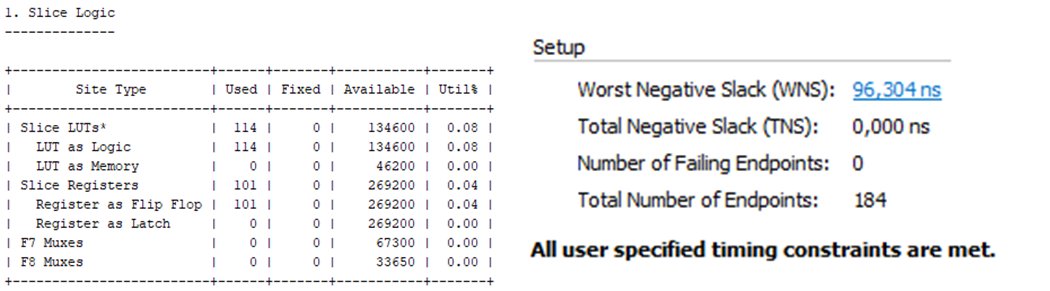
\includegraphics[keepaspectratio=true,scale=0.4]{images/Capitolo3/report.png}
    \caption{Il risultato dei report di Vivado}
    \label{fig:Report}
\end{figure}

In particolare il componente è composto da 101 Flip Flop, 0 latch e vengono utilizzati soli 4 nanosecondi a ogni ciclo di clock per completare le operazioni sui 100 disponibili.

\section{Test Benches}
Per verificare l’effettivo funzionamento del componente, esso è stato testato con numerosi test bench e con qualche test mirato sui casi critici nonostante la struttura del progetto non presenta molti corner case che non sono già richiesti all'interno della specifica. Qui di seguito si fornisce una breve descrizione dei casi più importanti.
\subsubsection{0 Byte da leggere}
Il caso in cui i Byte da leggere sono 0 il componente si comporta correttamente, esso non fa partire la convoluzione e termina il processo.
\begin{figure}[!htb]
    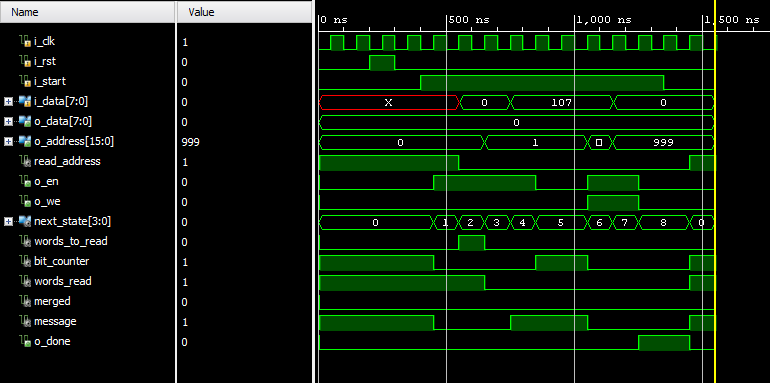
\includegraphics[keepaspectratio=true,scale=0.7]{images/Capitolo3/min.PNG}
    \caption{Lo schema dei segnali nel caso in cui non ci siano parole da leggere}
    \label{fig:signal1}
\end{figure}
\subsubsection{255 Byte da leggere}
Il caso in cui i Byte da leggere sono il massimo richiesto il componente non presenta criticità ed esegue la convoluzione correttamente.
\begin{figure}[!htb]
    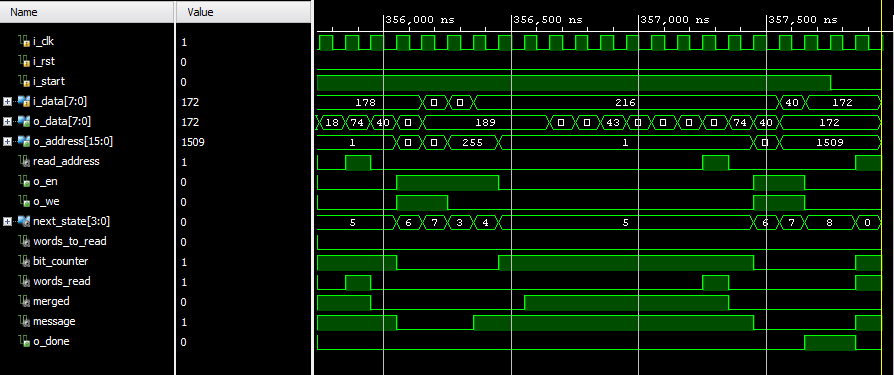
\includegraphics[keepaspectratio=true,scale=0.65]{images/Capitolo3/max.PNG}
    \caption{Lo schema dei segnali nel caso in cui la sequenza di parole da leggere è 255}
    \label{fig:signal2}
\end{figure}
\subsubsection{Due o più codifiche senza reset intermedio}
Nel caso in cui si vogliono eseguire più convoluzioni consecutive è necessario tenere conto che il componente deve essere pronto senza ricevere in ingresso un segnale di reset. Il componente realizzato rispetta la specifica e non ha problemi a gestire convoluzioni multiple.
\begin{figure}[!htb]
    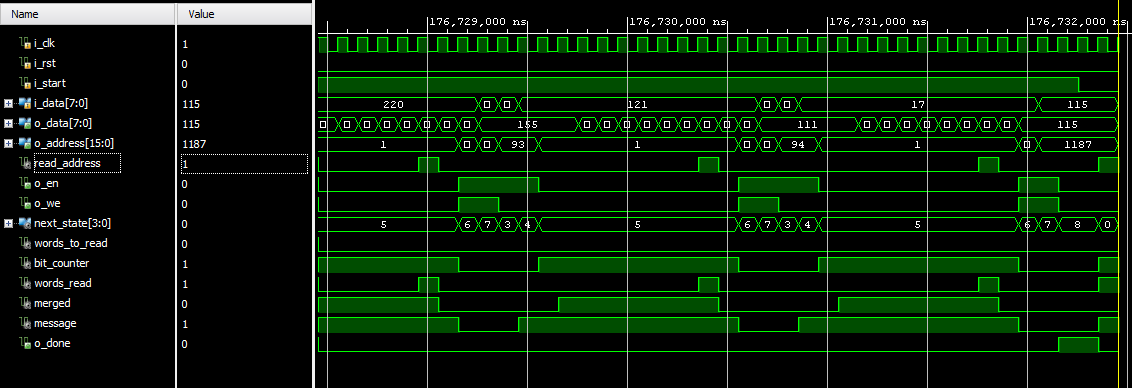
\includegraphics[keepaspectratio=true,scale=0.5]{images/Capitolo3/noreset.PNG}
    \caption{Lo schema dei segnali in un caso di codifiche multiple}
    \label{fig:signal3}
\end{figure}

\section{Conclusioni e Scelte Progettuali}
Si è giunti quindi alla conclusione che il componente realizzato rispetta pienamente le specifiche ed è stato accuratamente testato.

Si è deciso di utilizzare un registro per memorizzare l’indirizzo in cui leggere, e di non memorizzare quello in cui scrivere poiché viene ricavato in fase di esecuzione. Questo permette di avere un architettura più chiara e di risparmiare sull’utilizzo di qualche registro.
\include{chapters/Capitolo4}


\end{document}
% -----------------------------------------------------------------
